%!TEX root =  main.tex

\lectureheader{162}{Calculus II}{Applications of Taylor series}{\textit{Thomas' Calculus}  10.10}

\begin{definition}[Falling factorials]
Given $\alpha\in\R$ and a nonnegative integer $k$, $\alpha$ \textbf{falling} $k$ is the number
\begin{equation*}
\alpha^{\underline{k}} = \prod_{j=0}^{k-1}(\alpha-j).
\end{equation*}
\end{definition}
\begin{remark}\,
\begin{itemize}
\item By our convention that empty products are $1$, $\alpha^{\underline{0}}=1$ for all $\alpha$.
\item If $n$ is a nonnegative integer, then $n^{\underline{n}}=n!$.
\end{itemize}
\end{remark}


\begin{definition}[Binomial coefficients]
Given $\alpha\in\R$ and a nonnegative integer $k$, $\alpha$ \textbf{choose} $k$ is the number
\begin{equation*}
\binom{\alpha}{k} = \frac{\alpha^{\underline{k}}}{k!}
\end{equation*}
\end{definition}

\begin{example}
Compute $\binom{7}{3}$ and $\binom{4}{2}$.
Then compute $\binom{-1}{k}$ for all $k$.
\end{example}
\ifdefined\SOLUTION
\SOLUTION{
\begin{align*}
\binom{7}{3}&=\frac{7^{\underline{3}}}{3!}=\frac{7\cdot6\cdot5}{3\cdot2\cdot1}=35.\\
\binom{4}{2}&=\frac{4^{\underline{2}}}{2!}=\frac{4\cdot3}{2\cdot 1}=6.\\
\binom{-1}{k}&=\frac{(-1)^{\underline{k}}}{k!}=\frac{(-1)(-2)(-3)\cdots(-k)}{k!}=\frac{(-1)^k k!}{k!}=(-1)^k \quad (k\ge 0).
\end{align*}
} 
\fi
\newpage

\begin{theorem}[Newton's binomial theorem]
For any (fixed) $\alpha\in\R$,
\begin{equation*}
(1+x)^\alpha = \sum_{k=0}^\infty\binom{\alpha}{k}x^k
\end{equation*}
for all $-1< x< 1$.
\end{theorem}
\begin{remark}\,
\begin{itemize}
\item For some choices of $\alpha$, the above identity may hold for more values of $x$.
\item For example, if $\alpha$ is a nonnegative integer, the ``infinite series" on the right turns out to be a polynomial and the identity holds for all real $x$.
\end{itemize}
\end{remark}

\begin{example}
Use the above theorem to quickly compute the Taylor polynomial of order $4$ about $x=0$ for $f(x)=\sqrt{1+x}$.
\end{example}
\ifdefined\SOLUTION
\SOLUTION{
\begin{equation*}
    f(x) = (1+x)^{1/2} = \sum_{k=0}^\infty \binom{1/2}{k}x^k
\end{equation*}
\begin{align*}
 \binom{1/2}{0}&=1 \\
 \binom{1/2}{1}&=\frac{1/2}{1!}=\frac{1}{2},\\
 \binom{1/2}{2}&=\frac{(1/2)(-1/2)}{2!}=-\frac{1}{8},\\
 \binom{1/2}{3}&=\frac{(1/2)(-1/2)(-3/2)}{3!}=\frac{1}{16},\\ 
 \binom{1/2}{4}&=\frac{(1/2)(-1/2)(-3/2)(-5/2)}{4!}=-\frac{5}{128}.
\end{align*}
So, 
\begin{equation*}
f(x)=(1+x)^{1/2}
=\sum_{k=0}^\infty\binom{1/2}{k}x^k
=1+\frac{1}{2}x-\frac{1}{8}x^2+\frac{1}{16}x^3-\frac{5}{128}x^4+\dots.
\end{equation*}
It follows that
\begin{equation*}
    P_f(x; 4,0) = 1 + \frac{1}{2}x - \frac{1}{8}x^2 + \frac{1}{16}x^3 - \frac{5}{128}x^4.
\end{equation*}
}
\else
\fi
\newpage

\begin{example}
Use power series to evaluate $\DS\lim_{x\to 1}\frac{\ln x}{x-1}$.
\end{example}
\ifdefined\SOLUTION
\SOLUTION{
Taylor series are useful for ``seeing" and then resolving indeterminate forms.
The limit in question has the form ``0/0" as $x\to 1$.
We resolve the issue by expanding everything as a power series about $x=1$.
Recall that
\begin{equation*}
\ln(1+z)=\sum_{k=1}^\infty\frac{(-1)^{k+1}}{k}z^k\quad (-1< z\le 1).
\end{equation*}
Taking $x = 1+z$, this implies that
\begin{equation*}
\ln x=\sum_{k=1}^\infty \frac{(-1)^{k+1}}{k}(x-1)^k\quad (0 < x \le 2).
\end{equation*}
Therefore, as $x\to 1$,
\begin{equation*}
\begin{split}
\frac{\ln{x}}{x-1}
&=\frac{(x-1)-\frac{1}{2}(x-1)^2+\frac{1}{3}(x-1)^3-\frac{1}{4}(x-1)^4+\dots}{x-1}\\
%&=\frac{(x-1)-(x-1)^2\left(\frac{1}{2}+\frac{1}{3}(x-1)-\frac{1}{4}(x-1)^2+\dots\right)}{x-1}\\
&=\frac{(x-1)+O\Big((x-1)^2\Big)}{x-1}\\
&=1+O(x-1).
\end{split}
\end{equation*}
In other words, near $x=1$ (but not at $x=1$), 
\begin{equation*}
\frac{\ln x}{x-1} \approx 1
\end{equation*}
with an error that is at worst some constant multiple of $x-1$.
Whence,
\begin{equation*}
\lim_{x\to 1}\frac{\ln x}{x-1}
=\lim_{x\to 1}\Big(1+O(x-1)\Big)
=1.
\end{equation*}
}
\fi
\newpage

\begin{remark}\,
\begin{itemize}
\item The figure below illustrates the fact proven in the previous exercise, namely,
\begin{equation*}
\frac{\ln x}{x-1} = 1 + O(x-1) \text{ as } x\to 1.
\end{equation*}
\item In particular, the plot suggests that if $0<|x-1|<5/8$, then
\begin{equation*}
\frac{\ln x}{x-1} \approx 1
\end{equation*}
with an error that is no worse than $|x-1|$.
\end{itemize}
\end{remark}

\begin{figure}[H]
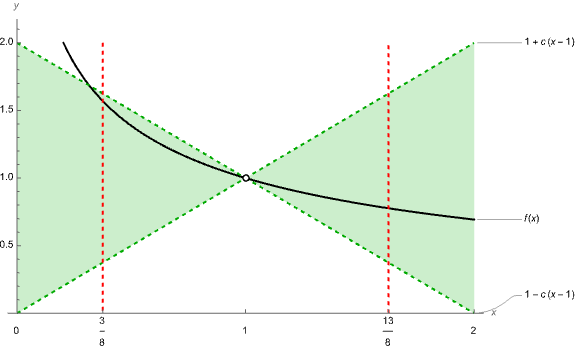
\includegraphics[width=6.5in]{img/power_series_and_limits1}
\caption{$f(x)=\DS\frac{\ln x}{x-1} = 1 + O(x-1)$ as $x\to 1$.}
\end{figure}

\newpage

\begin{example}
Use power series to evaluate the ``\textit{Mean Girls} limit"
$\DS\lim_{x\to 0}\frac{\ln(1-x)-\sin x}{1-\cos^2 x}$.
\end{example}
\ifdefined\SOLUTION
\SOLUTION{
Since the limit is indeterminate as $x\to 0$, we try expanding numerator and denominator as power series about $x=0$.
Recalling that
\begin{equation*}
\ln(1+x)=\sum_{k=1}^\infty(-1)^{k+1}\frac{x^k}{k}\quad (-1<x\le 1),
\end{equation*}
we deduce that
\begin{equation*}
\ln(1-x)=\sum_{k=1}^\infty(-1)^{k+1}\frac{(-x)^k}{k}
=-\sum_{k=1}^\infty\frac{x^k}{k}
\quad (-1\le x< 1).
\end{equation*}
Since 
\begin{equation*}
\sin x=\sum_{n=0}^\infty(-1)^n\frac{x^{2n+1}}{(2n+1)!}\quad (-\infty<x<\infty),
\end{equation*}
it follows that
\begin{equation*}
\ln(1-x)-\sin x=\left(-x-\frac{1}{2}x^2-\dots\right) - \left(x-\frac{1}{6}x^3+\dots\right)
=-2x+O(x^2)
\end{equation*}
as $x\to 0$.
Furthermore,
\begin{equation*}
\begin{split}
1-\cos^2(x)
=\sin^2(x)
&=\left(x-\frac{x^3}{6}+\dots\right)\left(x-\frac{x^3}{6}+\dots\right)\\
&=x^2 -\frac{1}{3}x^4+\dots\\
&=x^2+O(x^4)
\end{split}
\end{equation*}
as $x\to 0$.
Whence,
\begin{equation*}
\frac{\ln(1-x)-\sin x}{1-\cos^2 x}=\frac{-2x+O(x^2)}{x^2+O(x^4)}
=\frac{x}{x^2}\left(\frac{-2+O(x)}{1+O(x^2)}\right)
=\frac{1}{x}\left(\frac{-2+O(x)}{1+O(x^2)}\right)
\end{equation*}
as $x\to 0$, and therefore,
\begin{equation*}
\lim_{x\to 0}\frac{\ln(1-x)-\sin x}{1-\cos^2 x}
=\lim_{x\to 0}\frac{1}{x}\left(\frac{-2+O(x)}{1+O(x^2)}\right)\quad \text{DNE}.
\end{equation*}
}
\fi
\newpage

\begin{remark}\,
\begin{itemize}
\item The figure below illustrates a slightly stronger fact than what we proved in the previous exercise, namely,
\begin{equation*}
\frac{\ln(1-x)-\sin x}{1-\cos^2 x} = -\frac{2}{x} + O(1) \text{ as } x\to 0.
\end{equation*}
\item In particular, the plot suggests that if $0<|x|<3/4$, then
\begin{equation*}
\frac{\ln(1-x)-\sin x}{1-\cos^2 x} \approx -\frac{2}{x}
\end{equation*}
with an absolute error that is no worse than $2$.
\end{itemize}
\end{remark}

\begin{figure}[H]
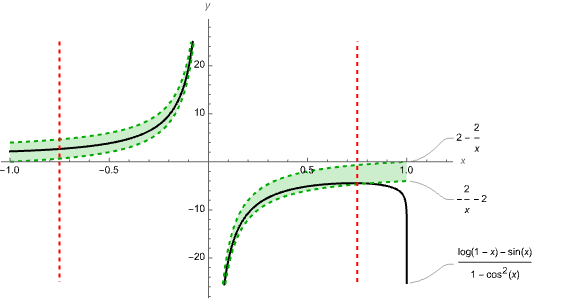
\includegraphics[width=6.5in]{img/power_series_and_limits2}
\caption{$f(x) =\DS\frac{\ln(1-x)-\sin x}{1-\cos^2 x} = -\frac{2}{x} + O(1)$ as $x\to 0$.}
\end{figure}

\newpage

\begin{remark}\,
\begin{itemize}
\item The classical (Newtonian) definition of the kinetic energy $K$ of an object with (a constant) mass $m$ moving with velocity $v$ is
\begin{equation*}
K= \frac{1}{2}mv^2.
\end{equation*}
\item In the modern (Einsteinian) theory, the \textit{relativistic mass} of an object is a function of its velocity, viz.,
\begin{equation*}
m = \frac{m_0}{\sqrt{1-(v/c)^2}},
\end{equation*}
where $m_0$ is the \textit{rest mass} and $c$ is the speed of light (both of which are constant/invariant in every frame of reference).
\item The kinetic energy of the object is then redefined to be
\begin{equation*}
K = (m-m_0)c^2.
\end{equation*}
\end{itemize}
\end{remark}

\begin{theorem}
As $v/c\to 0$,
\begin{equation*}
K = \frac{1}{2}m_0v^2 + O\bigg((v/c)^4\bigg).
\end{equation*}
\end{theorem}
\begin{remark}
In other words, if the velocity $v$ of the object is very small compared to the speed of light $c$, then the classical definition of kinetic energy is a good approximation to the modern definition in the sense that the error goes to zero (rather quickly) as $v/c\to 0$.
\end{remark}
\ifdefined\SOLUTION
\SOLUTION[Proof]{
The binomial theorem tell us that 
\begin{equation*}
\frac{1}{\sqrt{1+x}}=(1+x)^{-1/2}=\sum_{k=0}^\infty\binom{-1/2}{k}x^k\quad (-1 < x < 1),
\end{equation*}
and so if $-1<x<1$, then
\begin{equation*}
\frac{1}{\sqrt{1-x^2}}=\sum_{k=0}^\infty \binom{-1/2}{k}(-x^2)^k
=\sum_{k=0}^\infty (-1)^k\binom{-1/2}{k}x^{2k} 
=1+\frac{1}{2}x^2+\frac{3}{8}x^4+\dots
\end{equation*}
Whence, if $-1<v/c<1$, then
\begin{equation*}
m=\frac{m_0}{\sqrt{1-(v/c)^2}} 
=m_0+\frac{1}{2}m_0(v/c)^2+\frac{3}{8}m_0(v/c)^4+\dots.
\end{equation*}
Therefore, as $v/c\to 0$, we have
\begin{equation*}
m-m_0=\frac{1}{2}m_0(v/c)^2 + O\Big((v/c)^4\Big),
\end{equation*}
and hence
\begin{equation*}
K=(m-m_0)c^2=\frac{1}{2}m_0v^2+O\Big((v/c)^4\Big) 
\end{equation*}
as $v/c\to 0$.
}
\else
\begin{proof}
\,
\vspace{3.7in}

\end{proof}
\fi

\newpage


\begin{definition}
If $z$ is complex number, we define
\begin{equation*}
\exp(z) = \sum_{n=0}^\infty \frac{z^n}{n!}.
\end{equation*}
\end{definition}

\begin{theorem}[Euler's identity]
For any real number $\theta$,
\begin{equation*}
\exp(\I\theta) = \cos\theta + \I\sin\theta,
\end{equation*}
where $\I$ is a square root of $-1$, i.e, $\I^2=-1$.
\end{theorem}
\ifdefined\SOLUTION
\SOLUTION[Proof]{
Note that $\I^2=-1, \I^3=-i, \I^4=1, \I^5=i, \I^6=-1,\dots$.
So we should separate odd and even powered terms.  
Therefore, if $\theta$ is real, then 
\begin{align*}
\E^{\I\theta}&=\sum_{n=0}^\infty \frac{(\I\theta)^n}{n!}\\
&=\sum_{n=0}^\infty\frac{\I^n\theta^n}{n!}\\
&=\sum_{m=0}^\infty\frac{\I^{2m}\theta^{2m}}{(2m)!}+\sum_{m=0}^\infty \frac{\I^{2m+1}\theta^{2m+1}}{(2m+1)!}\\
&=\sum_{m=0}^\infty\frac{(-1)^{m}\theta^{2m}}{(2m)!}+\sum_{m=0}^\infty \frac{\I(-1)^{m}\theta^{2m+1}}{(2m+1)!}\\
&=\cos\theta+\I\sin\theta.
\end{align*}
}
\else
\begin{proof}
\,
\vspace{4.5in}

\end{proof}
\fi
\newpage

\begin{example}
Express $\DS\int\sin x^2\dee x$ as a power series.
Then estimate $\DS\int_0^1\sin x^2\dee x$ to within $10^{-3}$.
\end{example}
\ifdefined\SOLUTION
\SOLUTION{
For all $x\in\mathbb{R}$, 
\begin{align*}
\int \sin(x^2)\dee x &= \int \sum_{n=0}^\infty\frac{(-1)^n(x^2)^{2n+1}}{(2n+1)!}\dee x
= \sum_{n=0}^\infty\frac{(-1)^n}{(2n+1)!} \int x^{4n+2}\dee x \\
&=  C + \sum_{n=0}^\infty\frac{(-1)^n}{(2n+1)!}\cdot\frac{x^{4n+3}}{4n+3}.
\end{align*}
So,
\begin{equation*}
\int_0^1 \sin(x^2)\dee x 
= \left.\sum_{n=0}^\infty\frac{(-1)^n}{(2n+1)!}\cdot\frac{x^{4n+3}}{4n+3}\right|_0^1
= \sum_{n=0}^\infty\frac{(-1)^n}{(2n+1)!(4n+3)}.
\end{equation*}
By ASET,
\begin{equation*}
|R_N|=\left|\sum_{n=N+1}^\infty\frac{(-1)^n}{(2n+1)!(4n+3)}\right|
<\left|\frac{(-1)^{N+1}}{(2N+3)!(4N+7)}\right|
=\frac{1}{(2N+3)!(4N+7)}.
\end{equation*}
Observe that $|R_1| < \frac{1}{5!\cdot 11}\approx 0.00076 < 10^{-3}$.
Therefore,
\begin{equation*}
\int_0^1 \sin{(x^2)}\dee x \approx S_1 
=\sum_{n=0}^1\frac{(-1)^n}{(2n+1)!(4n+3)}
=\frac{1}{3} - \frac{1}{3!\cdot 7} 
=\frac{1}{3} - \frac{1}{42} 
=\frac{13}{42}
\end{equation*}
is accurate to within $10^{-3}.$
}
\else
\fi
